\documentclass[letter,12pt]{article}
\usepackage{fancyhdr}
\usepackage{amsmath}
\usepackage{amssymb}
\usepackage{bm}
\usepackage{synttree}
\usepackage[margin=1in]{geometry}
\usepackage{graphicx}
\pagestyle{fancy}
\lhead{Jesse Mu}
\rhead{CSCI339 Term Project}

\begin{document}

\title{How Are You Feeling? Analyzing Twitter User Mood with Naive Bayes
Sentiment Analysis}
\date{December 12, 2014}
\author{Jesse Mu}
\maketitle

\section{Background}

Sentiment analysis is a relatively new subset in the relatively new field of
machine learning but has since found significant research interest and
application in business analytics. Social networking site
Twitter\footnote{https://www.twitter.com/} has been identified as a key data
source to assist in sentiment analysis study. Given its status as one of the
biggest social networking sites in the world and its focus on trending topics
and discussion using hashtags, Twitter users' tweets represent a massive,
real-time snapshot of much of the world's opinions on countless topics---one of
the most valuable and accessible resources of its kind.

Sentiment analysis is an example of a machine learning classification problem.
As such, work in the field draws from standard classification models in the
literature (e.g. Support Vector Machines, Maximum Entropy Models, Naive Bayes
Classifiers) as applied to text classification \cite{pang02}. The fundamental
challenge of sentiment analysis is building a computer program that is able to
``learn'' from given data to generalize and form conclusions about new, unseen
examples. This can be successfully approached by the more standard supervised
(training data labeled with sentiment) approach or an unsupervised, lexical
(unlabeled training data) approach \cite{turney02}.

The classical application of sentiment analysis is opinion mining of movie
reviews, but the recent and dramatic surge in popularity of Twitter has
resulted in substantial research interest in the potential for usage of English
tweets as a corpus. Among the reasons for the usage of Twitter for sentiment
analysis provided by Pak and Paroubek \cite{pak10} are the inherent
subjectivity of social microblogging platforms, a large and incredibly varied
userbase, and potential for an ``arbitrarily large'' amounts of data.

When compared to other opinion mining tasks, sentiment analysis with a Twitter
corpus stands out because of the linguistic properties of its training
``documents.'' Tweets are incredibly short messages, with a 140-character
maximum limit, and encourage a fast, fundamentally electronic method of
communication. The casual, spontaneous, and compressed nature of the service
presents interesting and unique challenges. Specifically, feature extraction
has been the distinguishing area of research when dealing with tweets, as
researches encounter microblogging-specific problems including the usage of
emoticons, abbrevations, sarcasm, and the sheer brevity of the information
given.

Twitter sentiment analysis is not limited to the academic space. A critical
aspect of many companies' success is the successful monitoring and analysis of
subjective information on a product through social media, and sentiment
analysis on microblogging platforms plays a pivotal role. Because of the
uniqueness of its content, the issue of Twitter sentiment analysis has led
several companies to identify the problem as unique from standard sentiment
analysis programs, and some text analysis companies such as Datumbox employ a
separate Twitter analysis classification algorithm in addition to the
traditional classifier. In addition to Datumbox's API, several other commercial
services exist specifically for the sentiment analysis of English tweets. Many
o them are at least partially free to use, including
Sentiment140\footnote{http://www.sentiment140.com/},
Streamcrab\footnote{http://www.streamcrab.com/}, and
Semantria\footnote{https://semantria.com/}. A well-performing sentiment
analysis algorithm is a valuable asset, which motivates several of these
companies to keep their code closed-source, like Sentiment140 and Semantria.

\section{Problem Formulation}

\subsection{Corpus}
Because Twitter sentiment analysis is a relatively new
problem, there do not exist many good sources of labeled data for supervised
learning tasks. It is possible to train a classifier based on standard
sentiment data, e.g. from well-known movie review datasets, but the unique
terminology and writing style of tweets demands a native training corpus.

Previous papers have used smaller training sets such as the 2013 SemEval
corpus\footnote{http://www.cs.york.ac.uk/semeval-2013/task2/} ($\sim$9000
tweets) and the Sanders Analytics training
corpus\footnote{http://www.sananalytics.com/lab/twitter-sentiment/} ($\sim$5500
tweets) For this project, training data was taken from the Stanford
University-associated online tool Sentiment140 mentioned previously, which
provides a much larger corpus of 1,600,000 labeled tweets.

The sheer volume of tweets made available by Sentiment140 is due to the
automatic collection of tweets based on a simplifying assumption: any tweet
with positive emoticons (\texttt{:D}, \texttt{:)}, \texttt{=)}, etc) is labeled
as a positive tweet, and any tweet with negative emoticons (\texttt{:(},
\texttt{D:}, \texttt{=(}) is labeled as negative \cite{go09}. Intuitively, this
assumption seems reasonably valid; due to the short nature of tweets, those
with a positive emoticon are quite unlikely to have another negative emoticon
resulting in an overall negative sentiment. Of course, there are certainly
cases where this assumption fails, such as the usage of sarcasm and quoting.
Another disadvantage of this data set is that it makes no qualification based
on language; tweets of all languages are accepted, which decreases accuracy of
a solely English-based classifier. However, the sheer volume of this data set
outweighs other data sets by orders of magnitude and smooths out most anomalies.

\subsection{Naive Bayes}

Because the main area of focus in Twitter opinion
mining is good, reliable text preprocessing and feature extraction, multiple
classifiers were not considered. The best classification algorithm for
sentiment analysis tasks is disputed, and Go et al. \cite{go09} reports that
the optimal model is unclear, but one common, well-performing model suggested
by Gamallo \cite{gamallo14}, Narayanan \cite{narayanan13} and Pak \cite{pak10}
and used commercially by companies like Datumbox is the Naive Bayes classifier.

For each document $d$, Naive Bayes attempts to assign the class $c$ to $d$
where

\begin{equation}
  c = \max_{c_i} P(c_i | d)
\end{equation}

Bayes' Rule shows us that for each $c_i$, $P(c_i | d)$ is equivalent to

\begin{equation}
  P(c_i|d) = \frac{P(d | c_i)P(c_i)}{P(d)}.
\end{equation}

The Naive Bayes algorithm then makes several simplifying assumptions. Because
for each document $d$, $P(d)$ is constant, it can simply be ignored without
consequence. Furthermore, $P(d | c_i)$ is calculated by considering the
features of document $d$, $x$, where $x_1 x_2 x_3\dots x_i$ are individual
features. The Naive Bayes model \emph{naively} assumes independence of these
features, giving the simplified model

\begin{equation}
  P(c_j | d) = P(c_j) \prod P(x_i | c_j).
\end{equation}

Depending on whether or not we have a prior belief about the distribution of
classes $P(c_j)$, the Naive Bayes model can either take this prior belief into
account or learn from the training data class occurrences. If all classes are
equally likely, the term $P(c_j)$ becomes irrelevant.

There are many advantages of the Naive Bayes classifier, although of course
several disadvantages. Perhaps the benefit most tangible to this project is the
speed and simplicity of the Naive Bayes algorithm, which requires considerably
less time and memory consumption than similar classification algorithms such as
SVM and ensemble learning methods \cite{huang03}. Considering feature selection
is paramount, a fast algorithm allows for rapid experimentation and
prototyping, which makes detailed statistical analysis substantially easier.
Despite its arguably oversimplifying assumptions, Naive Bayes is uniquely good
at dealing with discrete text classification features, since more advanced
feature selection techniques such as n-grams can compensate. Again, although
disputed, Naive Bayes has been shown to outperform other algorithms in this
task \cite{narayanan13,pak10}.

Concerning disadvantages, one main issue with the Naive Bayes classifier is the
lack of a reliable confidence metric when making decisions on new documents.
Although the Naive Bayes classifier can output the probability it estimates for
each class, the classifier tends to be overconfident \cite{rennie01}. This can
pose problems when considering the web application in Section~\ref{sec:web}

There are two main variants of the Naive Bayes classifier used for
discrete data, Bernoulli and Multinomial, which will be discussed further.

\section{Technologies}

The full source code for this project is open-source and available on GitHub at the following
URL:
https://github.com/jayelm/TwitterSA.

The code is written exclusively in Python, selected primarily due to software
package availability. Text classification code uses the popular
scikit-learn\footnote{http://scikit-learn.org/stable/} machine learning library
which is built on the numpy\footnote{http://www.numpy.org/} and
scipy\footnote{http://www.scipy.org/} scientific computing stack. The result is
a heavily optimized machine learning library that retains the familiar and
intuitive Python syntax while resorting to C bindings and optimizations when
necessary for speed. It also incorporates many useful machine learning
utilities to help automate feature extraction, pipelining, and evaluation.

The web application uses the web framework
Flask\footnote{http://flask.pocoo.org/}, and incorporates the scikit classifier
module written for this project. Flask was chosen due to its minimalism, which
suited the small project at hand; as a microframework, an entire web
application can be written in only a few files, which is ideal for this
project's small, single-use goal.

The cloud hosting service Heroku is used to host the web application. A
development version is running at http://twittersa.herokuapp.com/.

There are also several utility scripts included in the project, written with
Python and Shell, which assist in data sanitization and scraping.

\section{Classifier Evaluation}

The biggest portion of this project was the one specifically concerned with the
natural language processing task at hand, and evaluation was integral to the
development of my classification script and classifiers. Specifically, my goal
was to consider several factors of a Naive Bayes classifier to identify a
configuration most suitable for a production environment. To that end, I first
and foremost attempted to maximize classification accuracy on test sets, while
keeping in mind other important factors like portability (running time, memory
constraints) and other metrics.

\subsection{Preprocessing and Feature Vectorization}

\subsubsection{Preprocessing}

Preprocessing refers to the regularization and normalization of documents to
reduce extraneous document information like punctuation, stopwords, etc. in an
attempt to eliminate the extraction of ``noisy'' features that can decrease
accuracy and performance.

For this task, I created a \texttt{preprocess} function in
\texttt{classifiers.py} that sanitized the document input. After tokenizing the
input with NLTK's \texttt{word\_tokenizer} method (more robust than scikit's),
I implemented the following steps common in most text preprocessing
implementations:

\begin{itemize}
  \item Make all words lowercase.
  \item Decode strings into unicode literals.
  \item Stem each word with the NLTK Porter Stemmer.
  \item Remove punctuation, including Twitter-specific \texttt{@} signs
    (``mentions''), \texttt{\#} signs (``hashtags''), and URL symbols.
\end{itemize}

There are also other issues unique to the language of Tweets that must
be dealt with appropriately. Specifically, this includes the following
implemented steps:

\begin{itemize}
  \item Expanding acronyms (lol, wtf, lmao, etc) using a list of slang words
    from http://www.noslang.com/.
    \begin{itemize}
      \item Since Noslang provides their dictionary freely on the website, but
        not in a computerized format, this required me to create the utility script
        \texttt{util/noslang\_scraper.py}, which visits every page on the
        Noslang website, converting it into a Python dictionary, and
        serializing it.
    \end{itemize}
  \item Removing the occurrences of two-or-more repeated characters to just
    two characters
    \begin{itemize}
      \item E.g. ``cooool'' $\rightarrow$ ``cool'', ``crazyyy'' $\rightarrow$
        ``crazyy''
      \item Duplicate characters cannot completely be removed since it's too
        difficult to know when letters are duplicated due to the correct
        spelling of a word (e.g. ``cool'') or emphasis (``crazyy''). Still,
        partial reduction is better than no reduction, and there may be value
        in differentiating between normal and emphasized uses of words.
    \end{itemize}
    \item Emoticons are not considered in this training set. They are
      automatically removed by the Sentiment140 training corpus since an
      emoticon is present in every single training example such that they would
      carry no real information.
    \item Emoji (Japanese characters, of which many contain emoticons and other
      subjective images) are considered implicitly, when possible, since a
      subset of Emoji are represented by Unicode characters. Since I deal with
      unicode literals in my preprocessing step, these characters do have
      sentiments and counts associated with them.
\end{itemize}


After the text has been preprocessed, each document must be converted into a
numerical vector to be processed efficiently by a classification algorithm.

\subsubsection{The Bag-Of-Words Model}
\label{ssub:the_bag_of_words_model}

The most commonly used feature vectorization technique when dealing with text
data is the bag-of-words model, which represents each document in a corpus as
the unordered bag of its words.

Specifically, for a training corpus that contains
$n$ globally unique words, a unique numerical index is assigned to each word, 0
through $n - 1$. Once this global tally of words is created, either with a
dictionary or by usage of a hash function, each document $d$ is represented by
a feature vector $x \in \mathbb{R}^n$, where each element $x_n$ stores the
occurrence count of the $n$th word in the given document.

This model works very well when used in tandem with a Naive Bayes classifier,
since such a classifier assumes independence of features and the bag-of-words
model similarly doesn't keep track of word ordering.

Feature vectors created using the bag-of-words method can either be discrete
counts or binary presence attributes, and results in different types of Naive
Bayes classifiers that are discussed in Section~\ref{sub:initial_evaluation}.

Scikit-learn provides the \texttt{CountVectorizer} class for keeping track of
the features and vectorizing a set of data. There are many feature extraction
parameters that can be fine-tuned to produce better performance.

\subsubsection{Laplace Smoothing}
\label{ssub:laplace_smoothing}

Laplace (+1) smoothing is implemented in the scikit Naive Bayes classifiers for
dealing with unknown words. Lidstone (+0.5) smoothing was considered briefly as
well, but appeared to have little to no effect on classifier metrics.

\subsection{Initial Evaluation: Bernoulli versus Multinomial Naive Bayes}
\label{sub:initial_evaluation}

There are two main types of Naive Bayes classifiers that handle discrete data,
and they make different assumptions about the probability distribution
underlying the data. The first is the Multinomial Naive Bayes algorithm, which
makes classification decisions assuming the features follow a multinomial
(polynomial) distribution, while the second is the Bernoulli Naive Bayes, which
makes classification decisions based on the Bernoulli (binary) probability
distribution. The main difference between the two is that the Multinomial Naive
Bayes considers the count of occurrences of a given word, rather than just its
presence. On the other hand, the Bernoulli Naive Bayes model works only with
binary features---it considers only the presence of given words. Scikit-learn
provides two classes, \texttt{MultinomialNB} and \texttt{BernoulliNB} that
implement these classifiers. Non-binary data given to a \texttt{BernoulliNB}
instance is binarized and treated like a binary distribution.

One imporant decision to make before continuing with analysis is whether to use
the Bernoulli or the Multinomial distribution. The easiest way to make this
decision is to simply compare the performance of bost on some naive, simple
implementation of the classifiers.

For this initial evaluation, I used a standard bag-of-words approach with my
preprocessing function. Training set size was broken into randomly sampled sets
from 100 to 25000 tweets. A standard Bernoulli or Multinomial Naive Bayes
classifier was run on a 70/30 train/test split, and was randomly sampled and
tested 5 times to reduce the variance with test set selection.
Figure~\ref{fig:bow_bernoulli_vs_multinomial} shows both the accuracy and
$F$-score performance metrics for Bernoulli and Multinomial Naive Bayes
classifiers based on varying training sets.

\begin{figure}[h]
  \centering
  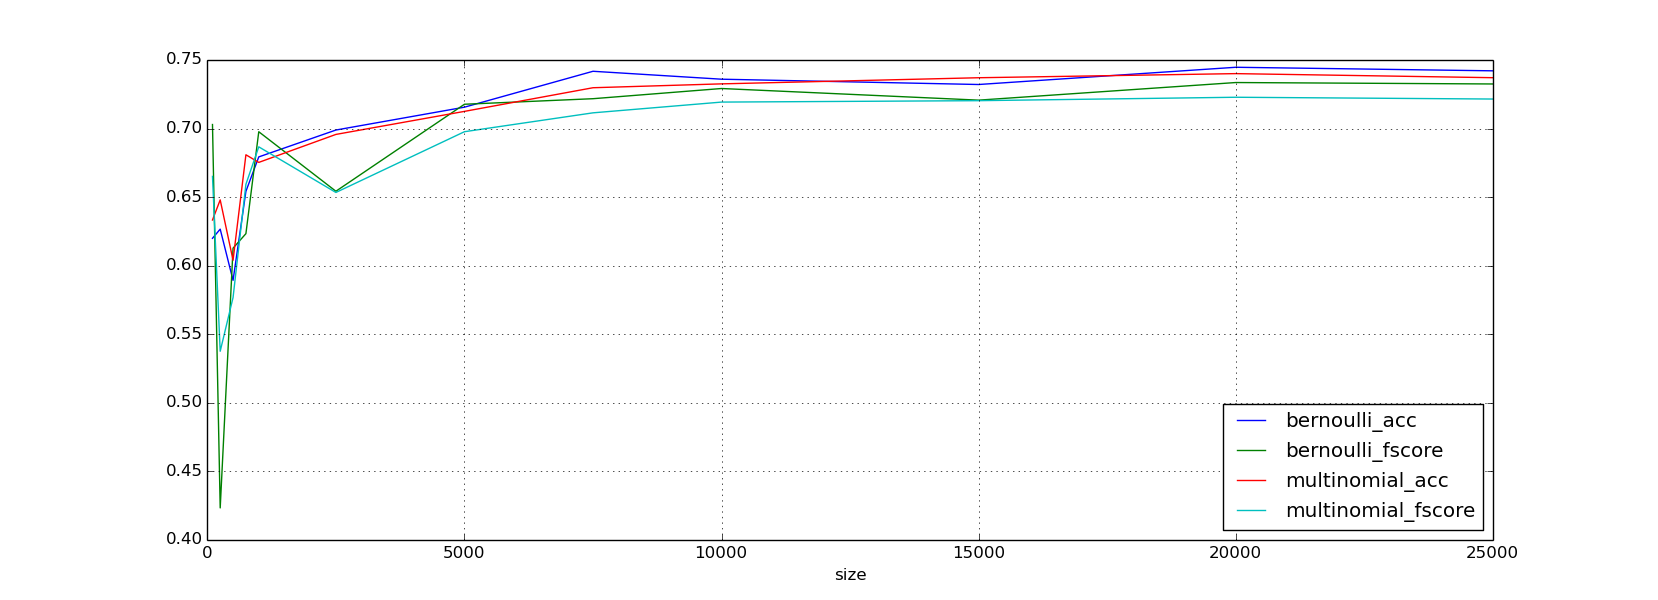
\includegraphics[width=\linewidth]{img/bow_bernoulli_vs_multinomial.png}
  \caption{Bernoulli vs Multinomial NB plotted against data set size}
  \label{fig:bow_bernoulli_vs_multinomial}
\end{figure}

As evidenced from Figure~\ref{fig:bow_bernoulli_vs_multinomial}, the difference
between a Bernoulli and Multinomial distribution is very little, with the
Bernoulli accuracy and $F$-score just slightly outperforming the multinomial
metrics with data set of sizes 15,000+, with peak accuracy achieved by the
Binomial Naive Bayes classifier at 74.21\%. This is a good accuracy achieved
with considering very standard implementation details.

The small difference between the Bernoulli and Multinomial distributions is
attributed to the short nature of Tweets. Multinomial classifiers take counts
of words into account, with multiple words carrying higher weight than singular
words. However, since Tweets are very short, multiple word occurrences do not
occur often enough for sufficient information to be gained from considering
multiple counts.

One other interesting thing to note is the effect of data size on
classification accuracy. Although accuracy rises rapidly when dealing with
smaller data sets (from $\sim$55\% accuracy to $\sim$75\%), the classifier
experiences diminishing returns when continuing to increase the data set size.
From initial evaluation, performance on the classifier seemed to flatten out
enough that a 25,000 tweet corpus was used as a good balance between accuracy
and speed for the tandard evaluation size for
the rest of the experiments conducted here. However, as we will see later,
greatly increasing data (by orders of magntiude) does continue to improve
classifier performance.

Since a Bernoulli Naive Bayes distribution is mildly more efficient, we will
continue using it alone, especially considering that the Bernoulli Naive Bayes
classifier is generally recommended over the Multinomial for short documents
\cite{manning08}.

\subsection{Improving Classification Accuracy}

The task at hand then becomes: how can we improve classification accuracy of
the model developed? With the selection of a Bernoulli Naive Bayes classifier,
the bulk of the potential for improvement lies in two main factors:

\begin{itemize}
  \item Improving feature extraction and selection
  \item Obtaining more data
\end{itemize}

\subsubsection{N-grams}
\label{ssub:n_grams}

The most basic NB classifier tested in the initial evaluation simply considers
all globally unique $n$ words as features. One way to potentially improve
classification accuracy is by including strings of words as features. For
example, ``The movie was not great'' can be broken down into bigrams ``The
movie'', ``movie was'', ``was not'', and ``not great''. Trigrams are similarly
constructed

The theoretical underpinning behind N-grams is that longer, combined sections
of words can capture more sophisticated language constructs than unigrams can.
Most notably, the inclusion of bigrams as features is one solution to the
negation problem, where the classifier can then consider directly negated
features, i.e. ``not good''. Of course, ``not'' and ``good'' are still
considered as unigram features, but the idea is that the presence of the bigram
would outweigh these two features. Furthermore, there is value in recognizing
the difference between ``somewhat good'' and ``extremely good'', two adjectives
that would be missed from unigram feature selection but included and
differentiated by bigrams.

These word-constructs are especially useful to Naive Bayes and bag-of-words
classifiers since they assume independence between all features. By including
ordered sections of words, N-grams add order considerations to the classifier,
not in the classification algorithm itself but the feature selection. As
displayed in Table~\ref{tab:ngrams}, accuracy gains are relatively minimal,
however, we see a jump of about 0.7\% accuracy when including bigrams. Trigrams
prove to overfit the data, and result in an accuracy reduction of 0.35\%; this
is probably due to the brevity of Tweets.

\begin{table}[h]
\centering
\begin{tabular}{c | c}
  N-grams & Accuracy \\
  \hline
  1 & 0.7408 \\
  2 & 0.7473 \\
  3 & 0.7448
\end{tabular}
\caption{Classifier accuracy for the cumulative addition of N-grams, 25000 data
set, averaged over 5 samples}
\label{tab:ngrams}
\end{table}

In scikit-learn, N-gram selection is implemented by setting the
\texttt{ngram\_range} variable during creation of the
\texttt{CountVectorizer}. \texttt{(1, 1)} is the default, with cumulative
bigrams and trigrams representd by \texttt{(1, 2)} and \texttt{(1, 3)}
respectively.

\subsubsection{Reducing features: select $k$-best}
\label{ssub:reducing_features_select_k_best}

With the improved model considering bigrams in addition to unigrams, one of the
ways commonly reported to increase accuracy is to actually \emph{remove}
features; in doing so, the classifier is able to eliminate ``noisy'' features.
Selecting the $k$-best features in a data set is an attempt to statistically
determine the most ``informative'' features, and use only those features.

``Noisy'' features are those features that are probably irrelevant to the
sentiment of a data, but information learned from a training corpus may still
associate a given sentiment for a word; for example, due to the occurrences of
the word ``sandwich'' in the training dataset, it may inadvertently carry a
negative sentiment, although intuition tells us that ``sandwich'' should be
neither a positive or a negative word. The goal of select $k$-best feature
selection is to remove words like these that may skew document predictions.

There are multiple ways to evaluate which features are the most informative,
including selection via mutual information, chi-squared statistical testing,
ANOVA filtering, and more. Manning \cite{manning08} recommends the
chi-squared ($\chi^2$) statistical test for feature selection on text
classification, which is implemented in scikit as
\texttt{sklearn.feature\_selection.chi2}, with the corresponding select
$k$-best implementation at \texttt{sklearn.feature\_selection. SelectKBest}.
The \texttt{SelectKBest} instance takes a vectorized 2D array of feature
vectors, where it applies a given statistical test to determine the
user-supplied $k$-best features, trimming the array down into an $m \times k$
matrix.

For the 25,000 tweet data set, there are around 140,000 unigram + bigram
features. Figure~\ref{fig:k_best} shows the effect of select $k$-best feature
selection on classifier accuracy, averaged over 5 splits, based on varying
amounts of $k$. Surprisingly, select $k$-best feature selection does not appear
to have a significant effect on classifier accuracy. Obviously, when the number
of features selected is very low (e.g. 10), there is not nearly enough
information to make reliabale decisions on the data, and the accuracy is very
low. However, anywhere in the area between 5,000 and 140,000 features, select
$k$-best feature selection has little-to-no effect on classifier accuracy.

\begin{figure}[h]
  \centering
  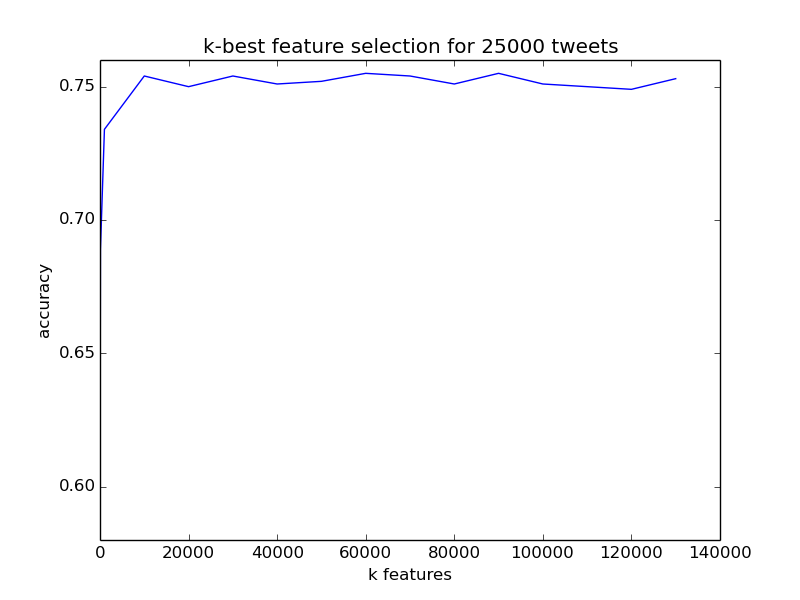
\includegraphics[width=0.8\linewidth]{img/k_best}
  \caption{Select $k$-best feature selection performance on 25000 data set
  (bigrams + unigrams), averaged over 5 splits}
  \label{fig:k_best}
\end{figure}

This is probably due to the fact that for bigger data sets and an equal
distribution of positive and negative cases, irrelevant words tend to appear
equally among both cases (i.e. the word ``the'' and ``sandwich'' should both
end up appearing in around 50\%
positive and negative cases). The Naive Bayes classifier is mathematically
insensitive to irrelevant features \cite{manning08}, so such features would not
have a big effect on classifier accuracy. Only on somewhat smaller data set sizes would
select $k$-best feature selection make a bigger difference in classifier
accuracy.
% Use the graph you had before

\subsubsection{Other Feature Selection Techniques}
\label{ssub:variance_threshold_feature_removal}

Both ``term inverse, inverse document frequency'' (TF-IDF) and variance
threshold removal feature selection techniques were considered, but neither
appeard to
have any tangible effect on classifier accuracy. TF-IDF is a
vector-transformation method that increases the importance of words depending on
how often they appear in a given document (TF) but downplays the importance of
words that appear several times in all documents (IDF). Because of the brevity
of the words in the Tweet corpus, TF-IDF does not have much effect on
classifier accuracy.

Variance threshold feature removal removes features whose variance does not
pass a certain threshold. Multiple thresholds were tested (0, 0.5, 1), but none
seemed to have a large effect.

% Do some tests

% Do some tests

\subsubsection{More Data - Diminishing Returns}
\label{ssub:more_data}

One of the use cases in which a Naive Bayes classifier is recommended is when
large amounts of data is available. A Naive Bayes classifier is crude but fast,
so it can take advantage of large amounts of data while still maintaining a
reasonable running time over comparable algorithms \cite{davis13}. As it turns
out, the single most effective way to increase test set accuracy on this
project is to greatly increase the amount of data. Although 25,000 was used as
the benchmark, Figure~\ref{fig:large_data_sets} shows the accuracy of a
classifier (with bigrams and 0.0 variance threshold feature removal) on data
sets at 25,000, 100,000, 250,000 and 500,000 tweets, averaged over 5 samples.
There is marked increase in classifier accuracy dependent on increasing size,
but at 500,000 tweets, memory and training time becomes an issue---the 500,000
tweet training set takes nearly 10 minutes to run and evaluate. A peak is
achieved for the 500,000 tweet data set at 79.12\%.

\begin{figure}[h]
  \centering
  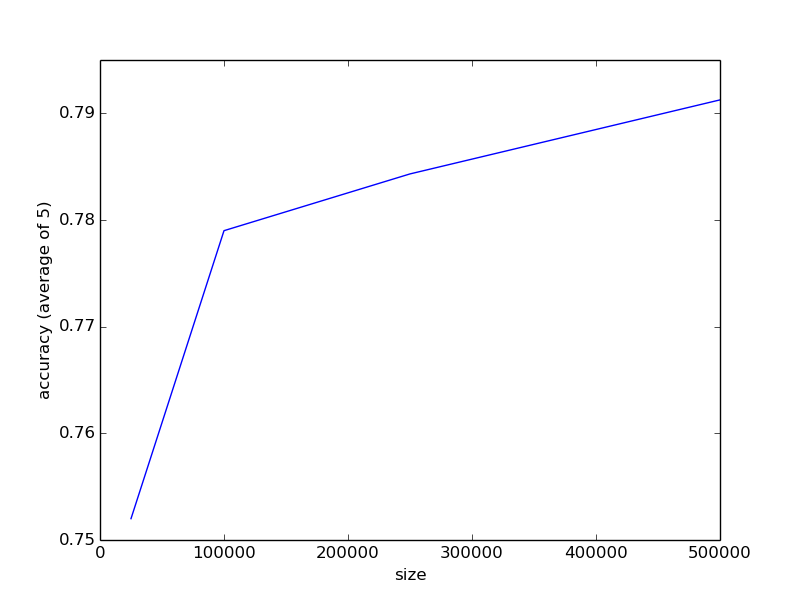
\includegraphics[width=0.8\linewidth]{img/large_data_sets.png}
  \caption{Effect of large training sets on classifier accuracy}
  \label{fig:large_data_sets}
\end{figure}


\section{Building the Web App}
\label{sec:web}

\subsection{Backend}

As previously mentioned, the web application was written in
Flask, and simply includes an index page, a user endpoint page, and an error
page. Most of the code is included in \texttt{TwitterSA.py}. When submitting a
request to the \texttt{/search?q=<USER-ID>} endpoint, the user function takes
the supplied Twitter username and attempts to get historical tweets associated
with that user by calling the \texttt{statuses/user\_timeline} Twitter API
endpoint. If no tweets are found, either because the user does not exist or the
timeline is private, an error page is shown.

How many tweets the application gets is dependent on the
\texttt{USER\_API\_CALLS} global variable set in \texttt{TwitterSA.py}. The API
enforces a limit of 200 tweets per user timeline call, and keeps a maximum
of up to 3200 tweets of historical data. Thus, this variable can be anywhere
from 1 to 16, and will attempt to get as many tweets as possible given the API
call limit.

The \texttt{status/user\_timeline} API endpoint is rate-limited to 300 requests
per minute for application-level authentication, so increasing
\texttt{USER\_API\_CALLS} results in quicker exhaustion of the rate allowance.
It is currently set at 2. The application currently uses a singular set of
Twitter API keys from an application registered at dev.twitter.com, since I do
not anticipate usage to be high enough such that the rate limit actually limits
usage of the application.

After tweets are collected, they are sorted by date and put into histogram-like
bins. Depending on the frequency of tweets, they are put into either weekly or
monthly time intervals. Then, the production classifier specified from
\texttt{sentiment/classifiers.py} predicts the sentiment for each tweet,
returning an array of \texttt{TweetSentiment} objects. The average sentiment
for each time interval is calculated, and transformed into a JSON-like object
that will be used for display by the frontend. Both this object and a list of
the original tweets are passed to the HTML view using the jinja2 templating
engine.

\subsection{Frontend}

Chart.js\footnote{http://www.chartjs.org/} is used as the visualization library
for the tweet information. It was selected over comparable libraries for
simplicity and ease of use, although it lacks the extensible functionality of
libraries like d3.js\footnote{http://d3js.org/}. The Python object containing
the \texttt{TweetSentiment} object is JSONified into a format understood by the
library, which creates the line plot plotting average Tweet sentiment against
each time interval. All tweets by the user are then displayed below the chart
with dates and individual sentiment probabilities. Some additional JavaScript
scripting is used to enable functionality, which is currently limited to
clicking on an individual node on the line chart and seeing the tweets specific
to that date range filtered under the chart. An example screenshot of this
library in action is located in Figure~\ref{fig:obama}.

\begin{figure}[h]
  \centering
  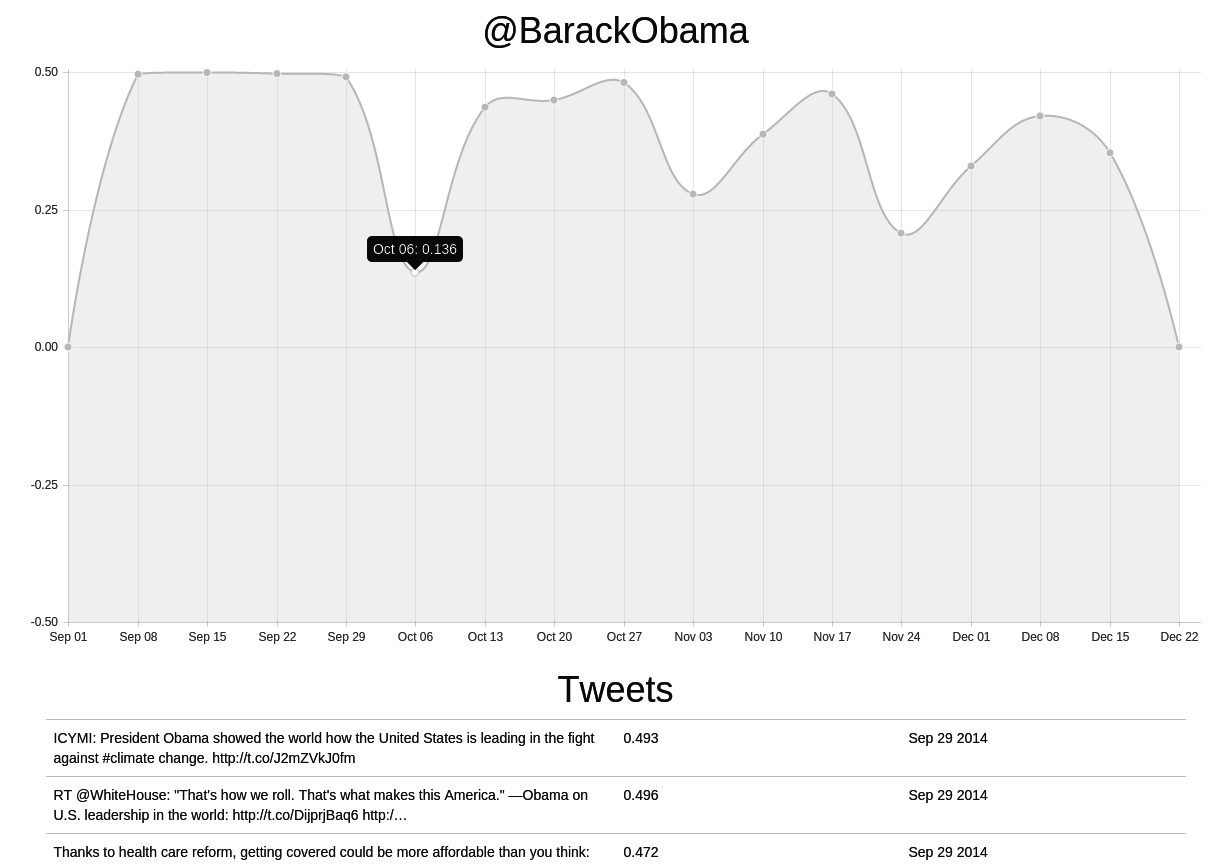
\includegraphics[width=0.8\linewidth]{img/obama_example_usage.png}
  \caption{Example Web Application Screenshot for Twitter User @BarackObama}
  \label{fig:obama}
\end{figure}

\section{Conclusions}

Using a standard Bernoulli Naive Bayes classification algorithm on the largest
500,000 tweet dataset (350,000/150,000 train/test split) with bigram feature
selection, the peak accuracy achieved by this classification system is 79.12\%.
This is a surprisingly good result that shows the efficacy of simple,
probabilistic machine learning techniques when applied to sentiment analysis.

Most notably, the task of sentiment analysis itself is
not a 100\% agreeable problem.  Specifically, Wilson et al. \cite{wilson05}, in
an empirical analysis, identified that when participants were asked to classify
sentences as ``positive'', ``neutral'', or ``negative'', only 82\% similarity
was recorded, not very far above the accuracy level recorded by this
classifier. When neutral tweets are removed, however, Wilson reported that
accuracy increased to $\sim$90\%. An $80\%$ benchmark by a machine, however, is
still quite good, and is comparable to the state-of-the-art work in statistical
sentiment analysis; Pang et al. \cite{pang02} report a maximum accuracy
percentage with a Naive Bayes classifier of 81.0\%.

There were of course several limitations to this study. Most of them were
mentioned during the writeup as I consider the implications of various
decisions used during the task. For example, the Sentiment140 dataset's
collection assumption could be inherently problematic (they are not
hand-classified), but the size of the training set outweighs this possible
disadvantage. Also, training data was taken from this same corpus. As such,
emoticons could not be considered, since they are removed from the original
Sentiment140 training set.

Since a Naive Bayes classifier is somewhat overconfident, using its probability
estimation as a ``confidence'' metric is somewhat problematic. This is somewhat
mitigated by the fact that the Flask application averages all of the
probabilities to gain a more global sentiment, but it is one of the inherent
weeknesses in a Naive Bayes classifier.

Notably, many feature selection techniques that were considered to work well
for text classification did not (especially the select $k$-best feature
selection). This could be indicative of an inherent issue with the subject
matter of the training corpus, and may need to be investigated further. Testing
on different, hand-tagged training sets, for example, may yield better results.

\paragraph{Ideas for Further Work}

Only a binary classifier was built, which distinguishes between positive and
negative examples. Since a NB classifier is somewhat overconfident on
decisions, including a neutral class may actually improve accuracy. This could
also improve the handling of decidedly netural tweets (e.g. ``I am eating a
sandwich''). Identifying neutrality could be done by making a probability
confidence threshold for polarity in the Naive Bayes classifier or other
methods implemented by Gamallo \cite{gamallo14} which first considers wheter or
not a tweet is Subjective or Objective before determining polarity.

With a bigger time investment, one interesting thing to do would be to look at
precision and recall metrics along with simple accuracy. This could give a more
sophisticated view of the performance of the classifier based on the different
properties selected.

More feature selection and preprocessing techniques could be considered; for
example, URLs can be normalized, instead of simply being stripped with
puncuation, and mentions and hashtags could simply be completely removed
instead of stripped of punctuation. A close analysis of accuracy would be
necessary to determine whether these changes would be beneficial for the
classifier. Narayanan \cite{narayanan13} also implements a negation
preprocessing step that prefixes negated words with \texttt{not\_}. Although I
implicitly try to amend this issue with N-gram feature selection, the negation
approach is certainly more sophisiticated and can probably result in better
analysis.

It also may be possible to include some discrete features separate from the
bag-of-words representation, including document length, number of ``polarized''
words according to a polarity lexicon, etc. These ideas are considered by
Gamallo \cite{gamallo14}. For tweets specifically, heuristic document features
like document length will probably not play a large role, althoguh a more
content-based approach could (with appropriate feature scaling) play a role.

And again, with more time and memory, further increasing data (up to
Sentiment140's 1,600,000 tweet corpus) will most likely further increase
accuracy. It may also be appropriate to examine other classification
algorithms, such as SVM or Ensemble methods, and make a comparative analysis.

\appendix
\section{Appendix: Python script help output}

\subsection{\texttt{classifiers.py}}
\label{sub:classifiers}

\begingroup
\fontsize{10pt}{12pt}\selectfont
\begin{verbatim}
usage: classifiers.py [-h] [-a] [-c CLASSIFIER] [-s] [-n NGRAM]
                      [--tf | --tfidf] [--show-best-features] [-k KBEST]
                      [-v [THRESHOLD]] [-p [PICKLE]] [-N NUM] [-r]
                      [corpus [corpus ...]]

positional arguments:
  corpus                corpus sizes (must be the size of a .pickle file in
                        lib/)

optional arguments:
  -h, --help            show this help message and exit
  -a, --all             grab all training .pickle files in lib
  -c CLASSIFIER, --classifier CLASSIFIER
                        specifiy classifier (bernoulli or multinomial)
  -s, --stopwords       filter out stopwords before processing
  -n NGRAM, --ngram NGRAM
                        use ngrams in addition to unigrams
  --tf                  use tf feature normalization
  --tfidf               use tf-idf feature normalization (incompatible with
                        --tf)
  -k KBEST, --k-best KBEST
                        select k best features with chi-squared statistical
                        test
  -v [THRESHOLD], --variance-threshold [THRESHOLD]
                        remove features with variance below threshold
  -p [PICKLE], --pickle [PICKLE]
                        save last classifier to given destination
  -N NUM, --num NUM     number of times to train each classifier
  -r, --repl            enter REPL for last classifier
\end{verbatim}
\endgroup

\subsection{\texttt{TwitterSA.py}}
\label{sub:twittersa}

\textbf{Note:} environment variables must be set before running the script.

\begingroup
\fontsize{10pt}{12pt}\selectfont
\begin{verbatim}
[2014-12-12 16:10:35,371] INFO in TwitterSA: Loading classifier...
[2014-12-12 16:10:57,365] INFO in TwitterSA: Done
usage: TwitterSA.py [-h] [-d]

optional arguments:
  -h, --help   show this help message and exit
  -d, --debug  run application in debug mode
\end{verbatim}
\endgroup


% \newpage

\begin{thebibliography}{9}

\bibitem{davis13}
  Davis, E. Naive Bayes for Classifying Text. Lecture notes from
  \emph{Introduction to Artificial Intelligence} (V22.0480.001, 2013), New York
  University.
  Retrieved from http://www.cs.nyu.edu/faculty/davise/ai/.

\bibitem{gamallo14}
  Gamallo, P., and Garcia, M. Citius: A Naive-Bayes Strategy for Sentiment
  Analysis on English Tweets. In \emph{Proceedings of the 8th International
  Workshop on Semantic Evaluation} (Dublin, Ireland, 2014), 171--175.

\bibitem{go09}
  Go, A., Bhayani, R.,  and Huang, L. Twitter Sentiment Classification using
  Distance Supervision. In \emph{Processing} (2009), 1--6.

\bibitem{huang03}
  Huang, J., Lu, J., and Ling, C. X. Comparing Naive Bayes, Decision Trees, and
  SVM with AUC and Accuracy. In \emph{The Third IEEE International Conference
  on Data Mining} (Melbourne, FL, 2003), 553--556.

\bibitem{manning08}
  Manning, C., Raghavan, P., and Schütze, H. /emph{Introduction to Information
  Retrieval}. Cambridge University Press, Cambridge, 2008.

\bibitem{narayanan13}
  Narayanan, V., Arora, I., and Bhatia, A. Fast and accurate sentiment
  classification using an enhanced Naive Bayes model. In \emph{Intelligent Data
  Engineering and Automated Learning Lecture Notes in Computer Science} (2013),
  194--201.

\bibitem{pak10}
  Pak, A., and Paroubek, P. Twitter as a Corpus for Sentiment Analysis and
  Opinion Mining. In \emph{LREC} (Valletta, Malta, 2010), European Language
  Resources Association, 1320--1326.

\bibitem{pang02}
  Pang, B., Lee, L., and Vaithyanathan, S.
  Thumbs up? Sentiment Classification using Machine Learning Techniques.
  in \emph{Proceedings of EMNLP} (Philadelphia, PA, 2002), Association for
  Computational Linguistics, 79--86.

\bibitem{rennie01}
  Rennie, J. Improving Multi-class Text Classification with Naive Bayes.
  Master's Dissertation (Cambridge, MA, 2001), Massachusetts Institute of
  Technology.

\bibitem{turney02}
  Turney, P.
  Thumbs Up or Thumbs Down? Semantic Orientation Applied to
  Unsupervised Classification of Reviews.
  in \emph{Proceedings of the 40th Annual Meeting of the Association for
  Computational Linguistics} (Stroudsburg, PA, 2002), Association for
  Computational Linguistics, 417--424.

\bibitem{wilson05}
  Wilson, T., Wiebe, J., and Hoffman, P. Recognizing Contextual Polarity in
  Phrase-Level Sentiment Analysis. In \emph{Proceedings of HLT/EMNLP} (2005),
  Association for Computational Linguistics, 347--354.

\end{thebibliography}

\end{document}
